\documentclass[a4paper,12pt]{report}
\usepackage[catalan]{varioref}
\usepackage{setspace}
\usepackage[margin=2.54cm]{geometry}
\usepackage{pdfpages}
\usepackage[utf8]{inputenc}
\usepackage[catalan]{babel}
\usepackage{graphicx,subcaption}
\usepackage{graphics}
\usepackage{lscape}
\usepackage{pdflscape}
\usepackage{float}
\usepackage{textcomp}
\usepackage{amsmath}
\usepackage{hyperref}
\usepackage{subcaption}
\usepackage{pgfplots}
\usepackage{tikz}
\usepackage{fancyvrb}
\usepackage{parskip}
\usepackage{changepage}
\usepackage{enumitem}
\usepackage{tcolorbox}
\usepackage[all]{hypcap}
\usepackage{xcolor}
\usepackage{listings}
\definecolor{green}{HTML}{228B22}
\definecolor{orange}{HTML}{FFC107}
\usepackage{color}
\definecolor{dkgreen}{rgb}{0,0.6,0}
\definecolor{gray}{rgb}{0.5,0.5,0.5}
\definecolor{mauve}{rgb}{0.58,0,0.82}
\lstset{escapeinside={<@}{@>}}

\hypersetup{
    colorlinks,
    citecolor=black,
    filecolor=black,
    linkcolor=black,
    urlcolor=blue
}


\lstset{frame=tb,
    language=python,
    aboveskip=3mm,
    belowskip=3mm,
    showstringspaces=false,
    columns=flexible,
    basicstyle={\small\ttfamily},
    numbers=none,
    numberstyle=\tiny\color{gray},
    keywordstyle=\color{blue},
    commentstyle=\color{dkgreen},
    stringstyle=\color{mauve},
    breaklines=true,
    breakatwhitespace=true, tabsize=3
}
\title{
	\begin{center}
	\vspace{3cm}
	
\includegraphics[width=11cm, height=3cm]{images/Logo-uoc.png}
	\end{center}
	\begin{center}
	\line(1,0){400}
	\end{center}		
	TIPOLOGIA I CICLE DE VIDA DE LES DADES\\
	\vspace{2mm}
	\Large PAC2: Introducció a la neteja i anàlisi de dades\\
	\line(1,0){400}
	\vspace{2.5cm}
	}

\author{Marc Cervera Rosell \vspace{1cm}}


\date{Semestre: febrer 2025 - juny 2025\vspace{0.5cm} \\ Màster en ciència de dades}
\onehalfspacing

\begin{document}
\thispagestyle{empty}
	\begin{titlepage}
		\maketitle
		\thispagestyle{empty}
	\end{titlepage}
	\cleardoublepage
	\newpage

\thispagestyle{empty}
\tableofcontents
\thispagestyle{empty}
\listoffigures
\thispagestyle{empty}
\newpage
\pagenumbering{arabic}
%\thispagestyle{empty}
\section*{Exercici 1}
\addcontentsline{toc}{section}{Exercici 1}

\subsection*{Pregunta 1}
\addcontentsline{toc}{subsection}{Pregunta 1}
La reducció de la dimensionalitat consisteix a disminuir el nombre de paràmetres d'un \textit{dataset} mantenint aquella informació més important. Aquests mètodes es poden dividir en paramètrics i no paramètrics. Els primers estimen les dades amb un model i els segons no treballen amb models sinó que treballen directament sobre les dades que hi ha disponibles. Un exemple de reducció de la dimensionalitat seria aplicar la tècnica PCA (\textit{Principal Component Analysis}) en un sistema de reconeixement facial. Només es conservarien les característiques clau que permeten la identificació.\\
La reducció de la quantitat de dades consisteix a retallar la volumetria original de les dades per una volumetria menor, però que "expliqui" el mateix que les dades originals. És a dir, la reducció de quantitat de dades consisteix a agafar un subconjunt més petit de dades del \textit{dataset} original. Un exemple de reducció de dades podria ser el resultat de la següent consulta SQL:
\begin{lstlisting}
    SELECT TOP 10000 * FROM [schema].[taula]
\end{lstlisting}
Aquesta consulta retorna les 10000 primeres files d'una taula que pot tenir milions de registres.
\subsection*{Pregunta 2}
\addcontentsline{toc}{subsection}{Pregunta 2}
La primera tècnica de detecció de valors atípics és mitjançant el mètode del rang interquartílic (IQR). El rang interquartílic és la diferència entre el tercer quartil (Q3) i el primer (Q1). Per tant, tot valor fora del rang [Q1 - 1.5 * IQR, Q3 + 1.5 * IQR] serà considerat un \textit{outlier}.\\
El segon mètode és mitjançant els diagrames de caixa. Els diagrames de caixa mostren una representació gràfica de la distribució de les dades. Els valors atípics en aquest cas, són tots aquells punts que queden fora dels bigotis de la caixa.\\
El tercer mètode és la puntuació Z. La puntuació Z és una mesura estadística que indica quantes desviacions estàndard es troba un valor respecte a la mitjana de les dades. Amb la puntuació Z de cada valor calculada (funció \textit{zscore} en Python) es compara aquesta (en valor absolut) i si és major a 3 es considera un valor atípic.
\newpage
\textbf{Exemples:}\\
\underline{Diagrama de caixa}\\
\begin{figure}[h]
    \centering
    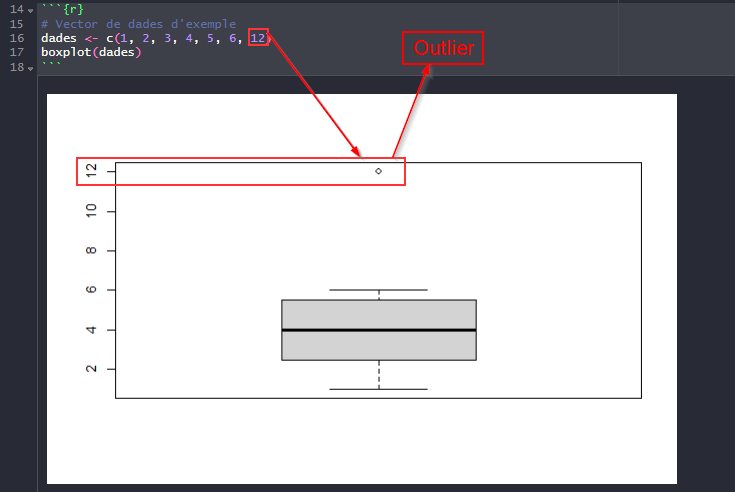
\includegraphics[scale=0.8]{images/boxplot.png}
    \caption{Exemple outlier diagrama de caixa}
    \label{fig:boxplot}
\end{figure}
\underline{IQR}\\
\begin{figure}[h]
    \centering
    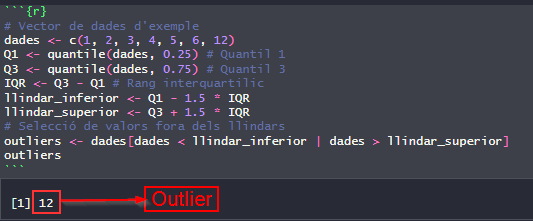
\includegraphics[scale=1]{images/iqr.png}
    \caption{Exemple outlier IQR}
    \label{fig:iqr}
\end{figure}
\underline{Puntuació Z}\\
\begin{figure}[h]
    \centering
    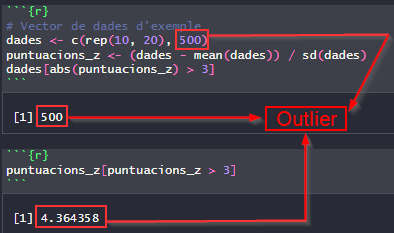
\includegraphics[scale=1]{images/z-scoring.png}
    \caption{Exemple outlier Z-scoring}
    \label{fig:zscoring}
\end{figure}
\section*{Exercici 2}
\addcontentsline{toc}{section}{Exercici 2}

\subsection*{Pregunta 1}
\addcontentsline{toc}{subsection}{Pregunta 1}

\subsection*{Pregunta 2}
\addcontentsline{toc}{subsection}{Pregunta 2}

\section*{Exercici 3}
\addcontentsline{toc}{section}{Exercici 3}

\subsection*{Pregunta 1}
\addcontentsline{toc}{subsection}{Pregunta 1}

\subsection*{Pregunta 2}
\addcontentsline{toc}{subsection}{Pregunta 2}

\section*{Exercici 4}
\addcontentsline{toc}{section}{Exercici 4}

\subsection*{Pregunta 1}
\addcontentsline{toc}{subsection}{Pregunta 1}

\subsection*{Pregunta 2}
\addcontentsline{toc}{subsection}{Pregunta 2}

\section*{Exercici 5}
\addcontentsline{toc}{section}{Exercici 5}

\subsection*{Pregunta 1}
\addcontentsline{toc}{subsection}{Pregunta 1}

\end{document}
